\documentclass[twoside]{book}

% Packages required by doxygen
\usepackage{fixltx2e}
\usepackage{calc}
\usepackage{doxygen}
\usepackage[export]{adjustbox} % also loads graphicx
\usepackage{graphicx}
\usepackage[utf8]{inputenc}
\usepackage{makeidx}
\usepackage{multicol}
\usepackage{multirow}
\PassOptionsToPackage{warn}{textcomp}
\usepackage{textcomp}
\usepackage[nointegrals]{wasysym}
\usepackage[table]{xcolor}

% Font selection
\usepackage[T1]{fontenc}
\usepackage[scaled=.90]{helvet}
\usepackage{courier}
\usepackage{amssymb}
\usepackage{sectsty}
\renewcommand{\familydefault}{\sfdefault}
\allsectionsfont{%
  \fontseries{bc}\selectfont%
  \color{darkgray}%
}
\renewcommand{\DoxyLabelFont}{%
  \fontseries{bc}\selectfont%
  \color{darkgray}%
}
\newcommand{\+}{\discretionary{\mbox{\scriptsize$\hookleftarrow$}}{}{}}

% Page & text layout
\usepackage{geometry}
\geometry{%
  a4paper,%
  top=2.5cm,%
  bottom=2.5cm,%
  left=2.5cm,%
  right=2.5cm%
}
\tolerance=750
\hfuzz=15pt
\hbadness=750
\setlength{\emergencystretch}{15pt}
\setlength{\parindent}{0cm}
\setlength{\parskip}{3ex plus 2ex minus 2ex}
\makeatletter
\renewcommand{\paragraph}{%
  \@startsection{paragraph}{4}{0ex}{-1.0ex}{1.0ex}{%
    \normalfont\normalsize\bfseries\SS@parafont%
  }%
}
\renewcommand{\subparagraph}{%
  \@startsection{subparagraph}{5}{0ex}{-1.0ex}{1.0ex}{%
    \normalfont\normalsize\bfseries\SS@subparafont%
  }%
}
\makeatother

% Headers & footers
\usepackage{fancyhdr}
\pagestyle{fancyplain}
\fancyhead[LE]{\fancyplain{}{\bfseries\thepage}}
\fancyhead[CE]{\fancyplain{}{}}
\fancyhead[RE]{\fancyplain{}{\bfseries\leftmark}}
\fancyhead[LO]{\fancyplain{}{\bfseries\rightmark}}
\fancyhead[CO]{\fancyplain{}{}}
\fancyhead[RO]{\fancyplain{}{\bfseries\thepage}}
\fancyfoot[LE]{\fancyplain{}{}}
\fancyfoot[CE]{\fancyplain{}{}}
\fancyfoot[RE]{\fancyplain{}{\bfseries\scriptsize Generated by Doxygen }}
\fancyfoot[LO]{\fancyplain{}{\bfseries\scriptsize Generated by Doxygen }}
\fancyfoot[CO]{\fancyplain{}{}}
\fancyfoot[RO]{\fancyplain{}{}}
\renewcommand{\footrulewidth}{0.4pt}
\renewcommand{\chaptermark}[1]{%
  \markboth{#1}{}%
}
\renewcommand{\sectionmark}[1]{%
  \markright{\thesection\ #1}%
}

% Indices & bibliography
\usepackage{natbib}
\usepackage[titles]{tocloft}
\setcounter{tocdepth}{3}
\setcounter{secnumdepth}{5}
\makeindex

% Hyperlinks (required, but should be loaded last)
\usepackage{ifpdf}
\ifpdf
  \usepackage[pdftex,pagebackref=true]{hyperref}
\else
  \usepackage[ps2pdf,pagebackref=true]{hyperref}
\fi
\hypersetup{%
  colorlinks=true,%
  linkcolor=blue,%
  citecolor=blue,%
  unicode%
}

% Custom commands
\newcommand{\clearemptydoublepage}{%
  \newpage{\pagestyle{empty}\cleardoublepage}%
}

\usepackage{caption}
\captionsetup{labelsep=space,justification=centering,font={bf},singlelinecheck=off,skip=4pt,position=top}

%===== C O N T E N T S =====

\begin{document}

% Titlepage & ToC
\hypersetup{pageanchor=false,
             bookmarksnumbered=true,
             pdfencoding=unicode
            }
\pagenumbering{alph}
\begin{titlepage}
\vspace*{7cm}
\begin{center}%
{\Large Project 1 \\[1ex]\large 1 }\\
\vspace*{1cm}
{\large Generated by Doxygen 1.8.12}\\
\end{center}
\end{titlepage}
\clearemptydoublepage
\pagenumbering{roman}
\tableofcontents
\clearemptydoublepage
\pagenumbering{arabic}
\hypersetup{pageanchor=true}

%--- Begin generated contents ---
\chapter{Project 1 File Parsing}
\label{index}\hypertarget{index}{}\begin{DoxyAuthor}{Author}
Kristopher Bickmore 
\end{DoxyAuthor}
\begin{DoxyDate}{Date}
November 20, 2016 
\end{DoxyDate}
\hypertarget{index_Build}{}\section{Build}\label{index_Build}
\hypertarget{index_Windows}{}\subsection{Windows}\label{index_Windows}
Tested on\+:~\newline
Windows 10 Pro 64-\/bit~\newline
Version 1607~\newline
OS Build 14393.\+447~\newline
 Microsoft Visual Studio Community 2015~\newline
Version 14.\+0.\+25431.\+01 Update 3\hypertarget{index_Linux}{}\subsection{Linux}\label{index_Linux}
Tested on\+:~\newline
Ubuntu 64-\/bit~\newline
Version 16.\+04.\+1 L\+TS xenial

G\+NU g++~\newline
Version 5.\+4.\+0 20160609

Eclipse~\newline
Version Neon.\+1a~\newline
Release 4.\+6.\+1~\newline
Build id\+: 20161007-\/1200

go to Project Properties -\/$>$ c/c++ Build -\/$>$ settings -\/$>$ Tool Settings -\/$>$ G\+CC C++ Compiler~\newline
Under Dialect select I\+SO c++1y(-\/std=c++1y)

go to Project Properties -\/$>$ c/c++ Build -\/$>$ settings -\/$>$ Tool Settings -\/$>$ G\+CC C++ Linker~\newline
Under Libraries add stdc++fs\hypertarget{index_MINGW32}{}\subsection{M\+I\+N\+G\+W32}\label{index_MINGW32}
There are bugs in the M\+I\+N\+G\+W32 compiler that mishandle c++11 functionality such as std\+::stoi or std\+::to\+\_\+string. \hypertarget{index_MINGW64}{}\subsection{M\+I\+N\+G\+W64}\label{index_MINGW64}
There are bugs in the M\+I\+N\+G\+W64 installer that did not allow me to ever properly install. Source code installation~\newline
failed do to missing libraries.~\newline
\hypertarget{index_Cygwin}{}\subsection{Cygwin}\label{index_Cygwin}
The Cygwin g++ compiler fails to properly resolve templates.~\newline
for instance passing a string into the path constructor does not resolve properly.~\newline
template$<$ class Source $>$~\newline
path( const Source\& source );~\newline
\hypertarget{index_Usage}{}\section{Usage}\label{index_Usage}
The program can be run with no options or a combination of the below.~\newline
~\newline
 Usage\+: parser(.exe) $<$option(s)$>$~\newline
 Lexer/\+Parser for files using the grammar specified for C\+M\+SC 330 Project 1.~\newline
~\newline
 Optional Options\+:~\newline
 -\/h,--help Show this help message.~\newline
 -\/d,--directory D\+I\+R\+E\+C\+T\+O\+RY Specify Path holding files to test. Cannot use with --file.~\newline
 (Defaults to ..\textbackslash{}test\+\_\+input\+\_\+files\textbackslash{} / ../test\+\_\+input\+\_\+files/)~\newline
 -\/o,--output D\+I\+R\+E\+C\+T\+O\+RY Specify Directory for output files.~\newline
 (Defaults to ..\textbackslash{}test\+\_\+input\+\_\+files\textbackslash{} / ../test\+\_\+input\+\_\+files/)~\newline
 -\/f,--file F\+I\+LE Use to Parse only a single file. Cannot use with --directory~\newline
 -\/p,--print Print output to screen.~\newline

\chapter{Bug List}
\label{bug}
\hypertarget{bug}{}

\begin{DoxyRefList}
\item[\label{bug__bug000001}%
\hypertarget{bug__bug000001}{}%
File \hyperlink{_lexer_8cpp}{Lexer.cpp} ]No known bugs at this time 
\end{DoxyRefList}
\chapter{Class Index}
\section{Class List}
Here are the classes, structs, unions and interfaces with brief descriptions\+:\begin{DoxyCompactList}
\item\contentsline{section}{\hyperlink{class_lexer}{Lexer} \\*This class is used to Lex a specific grammar\+: }{\pageref{class_lexer}}{}
\item\contentsline{section}{\hyperlink{class_parser}{Parser} \\*The parser class parses a specific grammar }{\pageref{class_parser}}{}
\item\contentsline{section}{\hyperlink{class_string_helper}{String\+Helper} \\*This class assists in handling std\+::string variables }{\pageref{class_string_helper}}{}
\end{DoxyCompactList}

\chapter{File Index}
\section{File List}
Here is a list of all documented files with brief descriptions\+:\begin{DoxyCompactList}
\item\contentsline{section}{C\+M\+S\+C330/\+Week4/\+P\+R\+O\+J\+E\+C\+T1/\hyperlink{_lexer_8cpp}{Lexer.\+cpp} \\*Contains the \hyperlink{class_lexer}{Lexer} class source code, which handles grammar lexing utilities }{\pageref{_lexer_8cpp}}{}
\item\contentsline{section}{C\+M\+S\+C330/\+Week4/\+P\+R\+O\+J\+E\+C\+T1/\hyperlink{_lexer_8h}{Lexer.\+h} \\*Contains the \hyperlink{class_lexer}{Lexer} class definition }{\pageref{_lexer_8h}}{}
\item\contentsline{section}{C\+M\+S\+C330/\+Week4/\+P\+R\+O\+J\+E\+C\+T1/\hyperlink{main_8cpp}{main.\+cpp} \\*The driver for the parser application }{\pageref{main_8cpp}}{}
\item\contentsline{section}{C\+M\+S\+C330/\+Week4/\+P\+R\+O\+J\+E\+C\+T1/\hyperlink{_parser_8cpp}{Parser.\+cpp} \\*Contains the source code for the \hyperlink{class_parser}{Parser} class }{\pageref{_parser_8cpp}}{}
\item\contentsline{section}{C\+M\+S\+C330/\+Week4/\+P\+R\+O\+J\+E\+C\+T1/\hyperlink{_parser_8h}{Parser.\+h} \\*Contains the \hyperlink{class_parser}{Parser} Class definition }{\pageref{_parser_8h}}{}
\item\contentsline{section}{C\+M\+S\+C330/\+Week4/\+P\+R\+O\+J\+E\+C\+T1/\hyperlink{stringhelper_8h}{stringhelper.\+h} \\*Contains the definition and source code for the \hyperlink{class_string_helper}{String\+Helper} class which provides extra string functionality }{\pageref{stringhelper_8h}}{}
\end{DoxyCompactList}

\chapter{Class Documentation}
\hypertarget{class_lexer}{}\section{Lexer Class Reference}
\label{class_lexer}\index{Lexer@{Lexer}}


This class is used to Lex a specific grammar\+:  




Collaboration diagram for Lexer\+:
\nopagebreak
\begin{figure}[H]
\begin{center}
\leavevmode
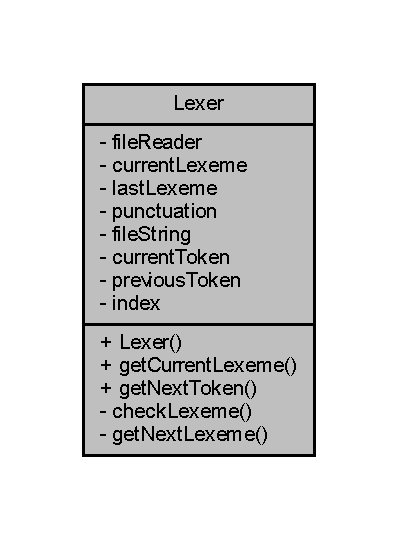
\includegraphics[width=191pt]{dd/d77/class_lexer__coll__graph}
\end{center}
\end{figure}
\subsection*{Public Member Functions}
\begin{DoxyCompactItemize}
\item 
\hyperlink{class_lexer_a41a25e738dff5c31caf442990709adde}{Lexer} (std\+::experimental\+::filesystem\+::path filename)  throw (std\+::runtime\+\_\+error)
\item 
std\+::string \hyperlink{class_lexer_a7fac880306793388754a6f9da34c3493}{get\+Current\+Lexeme} ()
\item 
\hyperlink{_lexer_8h_a6a9e93b081bad7fc74c17306fb168c1f}{Token} \hyperlink{class_lexer_aa8d555ee90674216793bb43c05bba64f}{get\+Next\+Token} ()
\end{DoxyCompactItemize}
\subsection*{Private Member Functions}
\begin{DoxyCompactItemize}
\item 
\hyperlink{_lexer_8h_a6a9e93b081bad7fc74c17306fb168c1f}{Token} \hyperlink{class_lexer_a50bcd81726a049971e16c4a6e8223604}{check\+Lexeme} (std\+::string lexeme)
\item 
std\+::string \hyperlink{class_lexer_a97988fed0390931fa45fe8a8fee39e2f}{get\+Next\+Lexeme} ()
\end{DoxyCompactItemize}
\subsection*{Private Attributes}
\begin{DoxyCompactItemize}
\item 
\hypertarget{class_lexer_adc8bdce9d027599208cd772a81b954d2}{}\label{class_lexer_adc8bdce9d027599208cd772a81b954d2} 
std\+::ifstream \hyperlink{class_lexer_adc8bdce9d027599208cd772a81b954d2}{file\+Reader}
\begin{DoxyCompactList}\small\item\em A file stream reading from the current file to be parsed. \end{DoxyCompactList}\item 
\hypertarget{class_lexer_aedfea368fa8e818b053df4f4cec803ba}{}\label{class_lexer_aedfea368fa8e818b053df4f4cec803ba} 
std\+::string \hyperlink{class_lexer_aedfea368fa8e818b053df4f4cec803ba}{current\+Lexeme}
\begin{DoxyCompactList}\small\item\em String which contains the lexeme currently being parsed/lexed. \end{DoxyCompactList}\item 
\hypertarget{class_lexer_a405095fbb33187d0cfff8b736970f4f1}{}\label{class_lexer_a405095fbb33187d0cfff8b736970f4f1} 
std\+::string \hyperlink{class_lexer_a405095fbb33187d0cfff8b736970f4f1}{last\+Lexeme}
\begin{DoxyCompactList}\small\item\em The string containing the lexeme that was previously looked at. \end{DoxyCompactList}\item 
\hypertarget{class_lexer_aab04ec42cbcd2e00f57fd4b9fd2255e4}{}\label{class_lexer_aab04ec42cbcd2e00f57fd4b9fd2255e4} 
std\+::string \hyperlink{class_lexer_aab04ec42cbcd2e00f57fd4b9fd2255e4}{punctuation}
\begin{DoxyCompactList}\small\item\em A string containing punctuation values which are delimiters in some way. \end{DoxyCompactList}\item 
\hypertarget{class_lexer_a8bec53e7c6adc2dd4f4ba5f6ac26d8b6}{}\label{class_lexer_a8bec53e7c6adc2dd4f4ba5f6ac26d8b6} 
std\+::string \hyperlink{class_lexer_a8bec53e7c6adc2dd4f4ba5f6ac26d8b6}{file\+String}
\begin{DoxyCompactList}\small\item\em String containing the text of the file. \end{DoxyCompactList}\item 
\hypertarget{class_lexer_af0484f3df6124444ce846bdfb5c0d14f}{}\label{class_lexer_af0484f3df6124444ce846bdfb5c0d14f} 
\hyperlink{_lexer_8h_a6a9e93b081bad7fc74c17306fb168c1f}{Token} \hyperlink{class_lexer_af0484f3df6124444ce846bdfb5c0d14f}{current\+Token}
\begin{DoxyCompactList}\small\item\em The token that is related to the current lexeme. \end{DoxyCompactList}\item 
\hypertarget{class_lexer_a6c351275177d71410545283a0d470021}{}\label{class_lexer_a6c351275177d71410545283a0d470021} 
\hyperlink{_lexer_8h_a6a9e93b081bad7fc74c17306fb168c1f}{Token} \hyperlink{class_lexer_a6c351275177d71410545283a0d470021}{previous\+Token}
\begin{DoxyCompactList}\small\item\em The token that is related to the prior lexeme. \end{DoxyCompactList}\item 
\hypertarget{class_lexer_aa7d95630ef9e53f6bdc5a9386420b343}{}\label{class_lexer_aa7d95630ef9e53f6bdc5a9386420b343} 
unsigned int \hyperlink{class_lexer_aa7d95630ef9e53f6bdc5a9386420b343}{index}
\begin{DoxyCompactList}\small\item\em Index into the file. \end{DoxyCompactList}\end{DoxyCompactItemize}


\subsection{Detailed Description}
This class is used to Lex a specific grammar\+:~\newline
 gui \+:\+:= Window S\+T\+R\+I\+NG \textquotesingle{}(\textquotesingle{} N\+U\+M\+B\+ER \textquotesingle{},\textquotesingle{} N\+U\+M\+B\+ER \textquotesingle{})\textquotesingle{} layout widgets End \textquotesingle{}.\textquotesingle{}~\newline
 layout \+:\+:= Layout layout\+\_\+type \textquotesingle{}\+:\textquotesingle{}~\newline
 layout\+\_\+type \+:\+:=~\newline
 Flow \textquotesingle{}(\textquotesingle{} \mbox{[} align \mbox{]} \textquotesingle{})\textquotesingle{}$\vert$~\newline
 Border \textquotesingle{}(\textquotesingle{} \mbox{[} N\+U\+M\+B\+ER \textquotesingle{},\textquotesingle{} N\+U\+M\+B\+ER \mbox{]} \textquotesingle{})\textquotesingle{}$\vert$~\newline
 Grid \textquotesingle{}(\textquotesingle{} N\+U\+M\+B\+ER \textquotesingle{},\textquotesingle{} N\+U\+M\+B\+ER \mbox{[}\textquotesingle{},\textquotesingle{} N\+U\+M\+B\+ER \textquotesingle{},\textquotesingle{} N\+U\+M\+B\+ER\mbox{]} \textquotesingle{})\textquotesingle{}~\newline
 align \+:\+:= L\+E\+FT $\vert$ R\+I\+G\+HT $\vert$ C\+E\+N\+T\+ER~\newline
 widgets \+:\+:= widget widgets $\vert$ widget~\newline
 widget \+:\+:=~\newline
 Button S\+T\+R\+I\+NG \textquotesingle{};\textquotesingle{} $\vert$~\newline
 Group radio\+\_\+buttons End \textquotesingle{};\textquotesingle{} $\vert$~\newline
 Label S\+T\+R\+I\+NG \textquotesingle{};\textquotesingle{} $\vert$~\newline
 Panel layout widgets End \textquotesingle{};\textquotesingle{} $\vert$~\newline
 Textfield N\+U\+M\+B\+ER \textquotesingle{};\textquotesingle{}~\newline
 radio\+\_\+buttons \+:\+:= radio\+\_\+button radio\+\_\+buttons $\vert$ radio\+\_\+button~\newline
 radio\+\_\+button \+:\+:= Radio S\+T\+R\+I\+NG \textquotesingle{};\textquotesingle{}~\newline


\subsection{Constructor \& Destructor Documentation}
\hypertarget{class_lexer_a41a25e738dff5c31caf442990709adde}{}\label{class_lexer_a41a25e738dff5c31caf442990709adde} 
\index{Lexer@{Lexer}!Lexer@{Lexer}}
\index{Lexer@{Lexer}!Lexer@{Lexer}}
\subsubsection{\texorpdfstring{Lexer()}{Lexer()}}
{\footnotesize\ttfamily Lexer\+::\+Lexer (\begin{DoxyParamCaption}\item[{std\+::experimental\+::filesystem\+::path}]{filename }\end{DoxyParamCaption}) throw  std\+::runtime\+\_\+error) }

\hyperlink{class_lexer}{Lexer} Constructor 
\begin{DoxyParams}{Parameters}
{\em filename} & the path to an input file to be lexed \\
\hline
\end{DoxyParams}
\begin{DoxyReturn}{Returns}
A \hyperlink{class_lexer}{Lexer} object 
\end{DoxyReturn}

\begin{DoxyExceptions}{Exceptions}
{\em runtime\+\_\+error} & \\
\hline
\end{DoxyExceptions}


\subsection{Member Function Documentation}
\hypertarget{class_lexer_a50bcd81726a049971e16c4a6e8223604}{}\label{class_lexer_a50bcd81726a049971e16c4a6e8223604} 
\index{Lexer@{Lexer}!check\+Lexeme@{check\+Lexeme}}
\index{check\+Lexeme@{check\+Lexeme}!Lexer@{Lexer}}
\subsubsection{\texorpdfstring{check\+Lexeme()}{checkLexeme()}}
{\footnotesize\ttfamily \hyperlink{_lexer_8h_a6a9e93b081bad7fc74c17306fb168c1f}{Token} Lexer\+::check\+Lexeme (\begin{DoxyParamCaption}\item[{std\+::string}]{lexeme }\end{DoxyParamCaption})\hspace{0.3cm}{\ttfamily [private]}}

Validates that the retrieved lexeme is a valid token. 
\begin{DoxyParams}{Parameters}
{\em lexeme} & a string to be compared against valid tokens \\
\hline
\end{DoxyParams}
\begin{DoxyReturn}{Returns}
The corresponding token 
\end{DoxyReturn}
\hypertarget{class_lexer_a7fac880306793388754a6f9da34c3493}{}\label{class_lexer_a7fac880306793388754a6f9da34c3493} 
\index{Lexer@{Lexer}!get\+Current\+Lexeme@{get\+Current\+Lexeme}}
\index{get\+Current\+Lexeme@{get\+Current\+Lexeme}!Lexer@{Lexer}}
\subsubsection{\texorpdfstring{get\+Current\+Lexeme()}{getCurrentLexeme()}}
{\footnotesize\ttfamily std\+::string Lexer\+::get\+Current\+Lexeme (\begin{DoxyParamCaption}{ }\end{DoxyParamCaption})}

Gets the lexeme that is currently being looked at. \begin{DoxyReturn}{Returns}
the lexeme 
\end{DoxyReturn}
\hypertarget{class_lexer_a97988fed0390931fa45fe8a8fee39e2f}{}\label{class_lexer_a97988fed0390931fa45fe8a8fee39e2f} 
\index{Lexer@{Lexer}!get\+Next\+Lexeme@{get\+Next\+Lexeme}}
\index{get\+Next\+Lexeme@{get\+Next\+Lexeme}!Lexer@{Lexer}}
\subsubsection{\texorpdfstring{get\+Next\+Lexeme()}{getNextLexeme()}}
{\footnotesize\ttfamily std\+::string Lexer\+::get\+Next\+Lexeme (\begin{DoxyParamCaption}{ }\end{DoxyParamCaption})\hspace{0.3cm}{\ttfamily [private]}}

Retrieves the next lexeme from the file. \begin{DoxyReturn}{Returns}

\end{DoxyReturn}
\hypertarget{class_lexer_aa8d555ee90674216793bb43c05bba64f}{}\label{class_lexer_aa8d555ee90674216793bb43c05bba64f} 
\index{Lexer@{Lexer}!get\+Next\+Token@{get\+Next\+Token}}
\index{get\+Next\+Token@{get\+Next\+Token}!Lexer@{Lexer}}
\subsubsection{\texorpdfstring{get\+Next\+Token()}{getNextToken()}}
{\footnotesize\ttfamily \hyperlink{_lexer_8h_a6a9e93b081bad7fc74c17306fb168c1f}{Token} Lexer\+::get\+Next\+Token (\begin{DoxyParamCaption}{ }\end{DoxyParamCaption})}

Retrieves the next token in the current line \begin{DoxyReturn}{Returns}
The Token 
\end{DoxyReturn}


The documentation for this class was generated from the following files\+:\begin{DoxyCompactItemize}
\item 
C\+M\+S\+C330/\+Week4/\+P\+R\+O\+J\+E\+C\+T1/\hyperlink{_lexer_8h}{Lexer.\+h}\item 
C\+M\+S\+C330/\+Week4/\+P\+R\+O\+J\+E\+C\+T1/\hyperlink{_lexer_8cpp}{Lexer.\+cpp}\end{DoxyCompactItemize}

\hypertarget{class_parser}{}\section{Parser Class Reference}
\label{class_parser}\index{Parser@{Parser}}


The parser class parses a specific grammar.  




Collaboration diagram for Parser\+:
\nopagebreak
\begin{figure}[H]
\begin{center}
\leavevmode
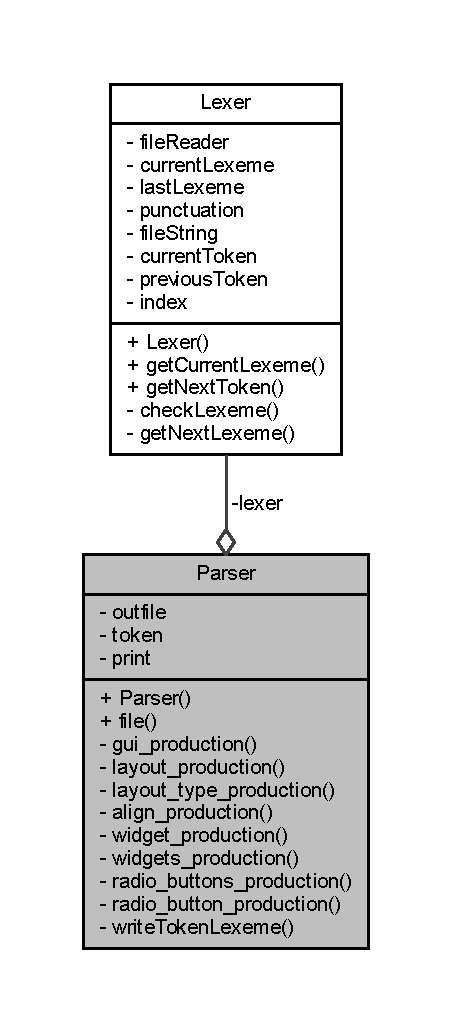
\includegraphics[width=217pt]{d0/d5d/class_parser__coll__graph}
\end{center}
\end{figure}
\subsection*{Public Member Functions}
\begin{DoxyCompactItemize}
\item 
\hyperlink{class_parser_a91939ccabb3a2337cd959386b36fc8b0}{Parser} (std\+::experimental\+::filesystem\+::path in\+Filename, std\+::string \hyperlink{class_parser_aa5fb86beefedf2e8bbefca807fc74bca}{outfile}, bool \hyperlink{class_parser_a127bec7e69bb49eadf9f935bd680fb6c}{print})  throw (std\+::runtime\+\_\+error)
\item 
void \hyperlink{class_parser_aa419c434b0e0def8c101bf906928a5ba}{file} ()
\end{DoxyCompactItemize}
\subsection*{Private Member Functions}
\begin{DoxyCompactItemize}
\item 
bool \hyperlink{class_parser_aa1ca665de0b8bb360a8bb084c4044861}{gui\+\_\+production} ()
\item 
bool \hyperlink{class_parser_a5edcbcd8826520596b79dae93096425d}{layout\+\_\+production} ()
\item 
bool \hyperlink{class_parser_a7a248c83d07922badb615458a943d5dc}{layout\+\_\+type\+\_\+production} ()
\item 
bool \hyperlink{class_parser_a7576c690add9d1f68a5781c8c240d6a1}{align\+\_\+production} ()
\item 
bool \hyperlink{class_parser_ac5fd99f9c1c8e4c72c04c0a4c58a5caf}{widget\+\_\+production} ()
\item 
bool \hyperlink{class_parser_a9d1dce16ca4c75ff9a3208cc8200dd23}{widgets\+\_\+production} ()
\item 
bool \hyperlink{class_parser_a3cd45dd7f2cf5d84955ac8efca423073}{radio\+\_\+buttons\+\_\+production} ()
\item 
bool \hyperlink{class_parser_a67083b88f1f2755a7ea81830524c1551}{radio\+\_\+button\+\_\+production} ()
\item 
void \hyperlink{class_parser_a70c67e7914ab1daad785f3d96ca40b6a}{write\+Token\+Lexeme} (\hyperlink{_lexer_8h_a6a9e93b081bad7fc74c17306fb168c1f}{Token} \hyperlink{class_parser_a77945ac7a42745c4655c2cfd0152c891}{token}, std\+::string lexeme)
\end{DoxyCompactItemize}
\subsection*{Private Attributes}
\begin{DoxyCompactItemize}
\item 
\hypertarget{class_parser_aa5fb86beefedf2e8bbefca807fc74bca}{}\label{class_parser_aa5fb86beefedf2e8bbefca807fc74bca} 
std\+::ofstream \hyperlink{class_parser_aa5fb86beefedf2e8bbefca807fc74bca}{outfile}
\begin{DoxyCompactList}\small\item\em The output file stream associated with the current \hyperlink{class_lexer}{Lexer} input file stream. \end{DoxyCompactList}\item 
\hypertarget{class_parser_aad05518621c5340d31f2b986a6467584}{}\label{class_parser_aad05518621c5340d31f2b986a6467584} 
\hyperlink{class_lexer}{Lexer} \hyperlink{class_parser_aad05518621c5340d31f2b986a6467584}{lexer}
\begin{DoxyCompactList}\small\item\em The lexer which will provide tokens and lexemes. \end{DoxyCompactList}\item 
\hypertarget{class_parser_a77945ac7a42745c4655c2cfd0152c891}{}\label{class_parser_a77945ac7a42745c4655c2cfd0152c891} 
\hyperlink{_lexer_8h_a6a9e93b081bad7fc74c17306fb168c1f}{Token} \hyperlink{class_parser_a77945ac7a42745c4655c2cfd0152c891}{token}
\begin{DoxyCompactList}\small\item\em A token whose value will be proviced by the \hyperlink{class_lexer}{Lexer} class. \end{DoxyCompactList}\item 
\hypertarget{class_parser_a127bec7e69bb49eadf9f935bd680fb6c}{}\label{class_parser_a127bec7e69bb49eadf9f935bd680fb6c} 
bool \hyperlink{class_parser_a127bec7e69bb49eadf9f935bd680fb6c}{print}
\begin{DoxyCompactList}\small\item\em This value indicates whether or not the parser will print its output. \end{DoxyCompactList}\end{DoxyCompactItemize}


\subsection{Detailed Description}
The \hyperlink{class_parser}{Parser} class is used to parse each Token created by the \hyperlink{class_lexer}{Lexer} class and to parse the overall syntax of the grammar\+:~\newline
 gui \+:\+:= Window S\+T\+R\+I\+NG \textquotesingle{}(\textquotesingle{} N\+U\+M\+B\+ER \textquotesingle{},\textquotesingle{} N\+U\+M\+B\+ER \textquotesingle{})\textquotesingle{} layout widgets End \textquotesingle{}.\textquotesingle{}~\newline
 layout \+:\+:= Layout layout\+\_\+type \textquotesingle{}\+:\textquotesingle{}~\newline
 layout\+\_\+type \+:\+:=~\newline
 Flow \textquotesingle{}(\textquotesingle{} \mbox{[} align \mbox{]} \textquotesingle{})\textquotesingle{}$\vert$~\newline
 Border \textquotesingle{}(\textquotesingle{} \mbox{[} N\+U\+M\+B\+ER \textquotesingle{},\textquotesingle{} N\+U\+M\+B\+ER \mbox{]} \textquotesingle{})\textquotesingle{}$\vert$~\newline
 Grid \textquotesingle{}(\textquotesingle{} N\+U\+M\+B\+ER \textquotesingle{},\textquotesingle{} N\+U\+M\+B\+ER \mbox{[}\textquotesingle{},\textquotesingle{} N\+U\+M\+B\+ER \textquotesingle{},\textquotesingle{} N\+U\+M\+B\+ER\mbox{]} \textquotesingle{})\textquotesingle{}~\newline
 align \+:\+:= L\+E\+FT $\vert$ R\+I\+G\+HT $\vert$ C\+E\+N\+T\+ER~\newline
 widgets \+:\+:= widget widgets $\vert$ widget~\newline
 widget \+:\+:=~\newline
 Button S\+T\+R\+I\+NG \textquotesingle{};\textquotesingle{} $\vert$~\newline
 Group radio\+\_\+buttons End \textquotesingle{};\textquotesingle{} $\vert$~\newline
 Label S\+T\+R\+I\+NG \textquotesingle{};\textquotesingle{} $\vert$~\newline
 Panel layout widgets End \textquotesingle{};\textquotesingle{} $\vert$~\newline
 Textfield N\+U\+M\+B\+ER \textquotesingle{};\textquotesingle{}~\newline
 radio\+\_\+buttons \+:\+:= radio\+\_\+button radio\+\_\+buttons $\vert$ radio\+\_\+button~\newline
 radio\+\_\+button \+:\+:= Radio S\+T\+R\+I\+NG \textquotesingle{};\textquotesingle{}~\newline


\subsection{Constructor \& Destructor Documentation}
\hypertarget{class_parser_a91939ccabb3a2337cd959386b36fc8b0}{}\label{class_parser_a91939ccabb3a2337cd959386b36fc8b0} 
\index{Parser@{Parser}!Parser@{Parser}}
\index{Parser@{Parser}!Parser@{Parser}}
\subsubsection{\texorpdfstring{Parser()}{Parser()}}
{\footnotesize\ttfamily Parser\+::\+Parser (\begin{DoxyParamCaption}\item[{std\+::experimental\+::filesystem\+::path}]{in\+Filename,  }\item[{std\+::string}]{outfile,  }\item[{bool}]{print }\end{DoxyParamCaption}) throw  std\+::runtime\+\_\+error) }

The \hyperlink{class_parser}{Parser} constructor 
\begin{DoxyParams}{Parameters}
{\em in\+Filename} & a path to the current file to be parsed and lexed \\
\hline
{\em outfile} & the name of the file which will contain the output of the parser \\
\hline
{\em print} & Print output or not \\
\hline
\end{DoxyParams}
\begin{DoxyReturn}{Returns}
A parser object 
\end{DoxyReturn}

\begin{DoxyExceptions}{Exceptions}
{\em runtime\+\_\+error} & \\
\hline
\end{DoxyExceptions}


\subsection{Member Function Documentation}
\hypertarget{class_parser_a7576c690add9d1f68a5781c8c240d6a1}{}\label{class_parser_a7576c690add9d1f68a5781c8c240d6a1} 
\index{Parser@{Parser}!align\+\_\+production@{align\+\_\+production}}
\index{align\+\_\+production@{align\+\_\+production}!Parser@{Parser}}
\subsubsection{\texorpdfstring{align\+\_\+production()}{align\_production()}}
{\footnotesize\ttfamily bool Parser\+::align\+\_\+production (\begin{DoxyParamCaption}{ }\end{DoxyParamCaption})\hspace{0.3cm}{\ttfamily [private]}}

Validates the align production syntax. \begin{DoxyReturn}{Returns}
true if syntax is valid, false otherwise 
\end{DoxyReturn}
\hypertarget{class_parser_aa419c434b0e0def8c101bf906928a5ba}{}\label{class_parser_aa419c434b0e0def8c101bf906928a5ba} 
\index{Parser@{Parser}!file@{file}}
\index{file@{file}!Parser@{Parser}}
\subsubsection{\texorpdfstring{file()}{file()}}
{\footnotesize\ttfamily void Parser\+::file (\begin{DoxyParamCaption}{ }\end{DoxyParamCaption})}

Begins the process of parsing the input file \hypertarget{class_parser_aa1ca665de0b8bb360a8bb084c4044861}{}\label{class_parser_aa1ca665de0b8bb360a8bb084c4044861} 
\index{Parser@{Parser}!gui\+\_\+production@{gui\+\_\+production}}
\index{gui\+\_\+production@{gui\+\_\+production}!Parser@{Parser}}
\subsubsection{\texorpdfstring{gui\+\_\+production()}{gui\_production()}}
{\footnotesize\ttfamily bool Parser\+::gui\+\_\+production (\begin{DoxyParamCaption}{ }\end{DoxyParamCaption})\hspace{0.3cm}{\ttfamily [private]}}

Validates the gui production syntax. \begin{DoxyReturn}{Returns}
true if syntax is valid, false otherwise 
\end{DoxyReturn}
\hypertarget{class_parser_a5edcbcd8826520596b79dae93096425d}{}\label{class_parser_a5edcbcd8826520596b79dae93096425d} 
\index{Parser@{Parser}!layout\+\_\+production@{layout\+\_\+production}}
\index{layout\+\_\+production@{layout\+\_\+production}!Parser@{Parser}}
\subsubsection{\texorpdfstring{layout\+\_\+production()}{layout\_production()}}
{\footnotesize\ttfamily bool Parser\+::layout\+\_\+production (\begin{DoxyParamCaption}{ }\end{DoxyParamCaption})\hspace{0.3cm}{\ttfamily [private]}}

Validates the layout production syntax. \begin{DoxyReturn}{Returns}
true if syntax is valid, false otherwise 
\end{DoxyReturn}
\hypertarget{class_parser_a7a248c83d07922badb615458a943d5dc}{}\label{class_parser_a7a248c83d07922badb615458a943d5dc} 
\index{Parser@{Parser}!layout\+\_\+type\+\_\+production@{layout\+\_\+type\+\_\+production}}
\index{layout\+\_\+type\+\_\+production@{layout\+\_\+type\+\_\+production}!Parser@{Parser}}
\subsubsection{\texorpdfstring{layout\+\_\+type\+\_\+production()}{layout\_type\_production()}}
{\footnotesize\ttfamily bool Parser\+::layout\+\_\+type\+\_\+production (\begin{DoxyParamCaption}{ }\end{DoxyParamCaption})\hspace{0.3cm}{\ttfamily [private]}}

Validates the layout type production syntax. \begin{DoxyReturn}{Returns}
true if syntax is valid, false otherwise 
\end{DoxyReturn}
\hypertarget{class_parser_a67083b88f1f2755a7ea81830524c1551}{}\label{class_parser_a67083b88f1f2755a7ea81830524c1551} 
\index{Parser@{Parser}!radio\+\_\+button\+\_\+production@{radio\+\_\+button\+\_\+production}}
\index{radio\+\_\+button\+\_\+production@{radio\+\_\+button\+\_\+production}!Parser@{Parser}}
\subsubsection{\texorpdfstring{radio\+\_\+button\+\_\+production()}{radio\_button\_production()}}
{\footnotesize\ttfamily bool Parser\+::radio\+\_\+button\+\_\+production (\begin{DoxyParamCaption}{ }\end{DoxyParamCaption})\hspace{0.3cm}{\ttfamily [private]}}

Validates the radio button production syntax. \begin{DoxyReturn}{Returns}
true if syntax is valid, false otherwise 
\end{DoxyReturn}
\hypertarget{class_parser_a3cd45dd7f2cf5d84955ac8efca423073}{}\label{class_parser_a3cd45dd7f2cf5d84955ac8efca423073} 
\index{Parser@{Parser}!radio\+\_\+buttons\+\_\+production@{radio\+\_\+buttons\+\_\+production}}
\index{radio\+\_\+buttons\+\_\+production@{radio\+\_\+buttons\+\_\+production}!Parser@{Parser}}
\subsubsection{\texorpdfstring{radio\+\_\+buttons\+\_\+production()}{radio\_buttons\_production()}}
{\footnotesize\ttfamily bool Parser\+::radio\+\_\+buttons\+\_\+production (\begin{DoxyParamCaption}{ }\end{DoxyParamCaption})\hspace{0.3cm}{\ttfamily [private]}}

Validates the radio buttons production syntax. \begin{DoxyReturn}{Returns}
true if syntax is valid, false otherwise 
\end{DoxyReturn}
\hypertarget{class_parser_ac5fd99f9c1c8e4c72c04c0a4c58a5caf}{}\label{class_parser_ac5fd99f9c1c8e4c72c04c0a4c58a5caf} 
\index{Parser@{Parser}!widget\+\_\+production@{widget\+\_\+production}}
\index{widget\+\_\+production@{widget\+\_\+production}!Parser@{Parser}}
\subsubsection{\texorpdfstring{widget\+\_\+production()}{widget\_production()}}
{\footnotesize\ttfamily bool Parser\+::widget\+\_\+production (\begin{DoxyParamCaption}{ }\end{DoxyParamCaption})\hspace{0.3cm}{\ttfamily [private]}}

Validates the widget production syntax. \begin{DoxyReturn}{Returns}
true if syntax is valid, false otherwise 
\end{DoxyReturn}
\hypertarget{class_parser_a9d1dce16ca4c75ff9a3208cc8200dd23}{}\label{class_parser_a9d1dce16ca4c75ff9a3208cc8200dd23} 
\index{Parser@{Parser}!widgets\+\_\+production@{widgets\+\_\+production}}
\index{widgets\+\_\+production@{widgets\+\_\+production}!Parser@{Parser}}
\subsubsection{\texorpdfstring{widgets\+\_\+production()}{widgets\_production()}}
{\footnotesize\ttfamily bool Parser\+::widgets\+\_\+production (\begin{DoxyParamCaption}{ }\end{DoxyParamCaption})\hspace{0.3cm}{\ttfamily [private]}}

Validates the widgets production syntax. \begin{DoxyReturn}{Returns}
true if syntax is valid, false otherwise 
\end{DoxyReturn}
\hypertarget{class_parser_a70c67e7914ab1daad785f3d96ca40b6a}{}\label{class_parser_a70c67e7914ab1daad785f3d96ca40b6a} 
\index{Parser@{Parser}!write\+Token\+Lexeme@{write\+Token\+Lexeme}}
\index{write\+Token\+Lexeme@{write\+Token\+Lexeme}!Parser@{Parser}}
\subsubsection{\texorpdfstring{write\+Token\+Lexeme()}{writeTokenLexeme()}}
{\footnotesize\ttfamily void Parser\+::write\+Token\+Lexeme (\begin{DoxyParamCaption}\item[{\hyperlink{_lexer_8h_a6a9e93b081bad7fc74c17306fb168c1f}{Token}}]{token,  }\item[{std\+::string}]{lexeme }\end{DoxyParamCaption})\hspace{0.3cm}{\ttfamily [private]}}

Writes the next token and lexeme to the output file, prints the output to screen if print is true. 
\begin{DoxyParams}{Parameters}
{\em token} & the available token \\
\hline
{\em lexeme} & the available lexeme \\
\hline
\end{DoxyParams}


The documentation for this class was generated from the following files\+:\begin{DoxyCompactItemize}
\item 
C\+M\+S\+C330/\+Week4/\+P\+R\+O\+J\+E\+C\+T1/\hyperlink{_parser_8h}{Parser.\+h}\item 
C\+M\+S\+C330/\+Week4/\+P\+R\+O\+J\+E\+C\+T1/\hyperlink{_parser_8cpp}{Parser.\+cpp}\end{DoxyCompactItemize}

\hypertarget{class_string_helper}{}\section{String\+Helper Class Reference}
\label{class_string_helper}\index{String\+Helper@{String\+Helper}}


This class assists in handling std\+::string variables.  




Collaboration diagram for String\+Helper\+:
\nopagebreak
\begin{figure}[H]
\begin{center}
\leavevmode
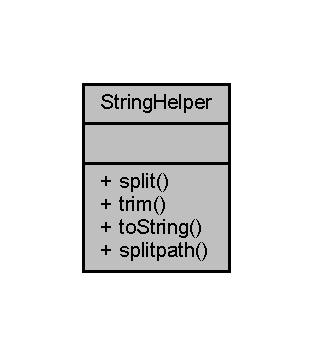
\includegraphics[width=150pt]{d4/d58/class_string_helper__coll__graph}
\end{center}
\end{figure}
\subsection*{Static Public Member Functions}
\begin{DoxyCompactItemize}
\item 
static std\+::list$<$ std\+::string $>$ \hyperlink{class_string_helper_a03cb28b0b0ced4aca4ccac59bdd74625}{split} (const std\+::string \&source, char delimiter)
\item 
static std\+::string \hyperlink{class_string_helper_a7861a9bf77dd724b5c046e34fe43eaa4}{trim} (const std\+::string \&s)
\item 
{\footnotesize template$<$typename T $>$ }\\static std\+::string \hyperlink{class_string_helper_a0a203a5eed0ff6d62b0a7530dee06386}{to\+String} (const T \&subject)
\item 
static std\+::vector$<$ std\+::string $>$ \hyperlink{class_string_helper_a783526b9f8fd876bddefd767537f49cf}{splitpath} (const std\+::string \&str, const std\+::set$<$ char $>$ delimiters)
\end{DoxyCompactItemize}


\subsection{Member Function Documentation}
\hypertarget{class_string_helper_a03cb28b0b0ced4aca4ccac59bdd74625}{}\label{class_string_helper_a03cb28b0b0ced4aca4ccac59bdd74625} 
\index{String\+Helper@{String\+Helper}!split@{split}}
\index{split@{split}!String\+Helper@{String\+Helper}}
\subsubsection{\texorpdfstring{split()}{split()}}
{\footnotesize\ttfamily static std\+::list$<$std\+::string$>$ String\+Helper\+::split (\begin{DoxyParamCaption}\item[{const std\+::string \&}]{source,  }\item[{char}]{delimiter }\end{DoxyParamCaption})\hspace{0.3cm}{\ttfamily [inline]}, {\ttfamily [static]}}

Splits a string into multiple strings at each location of the given delimiter. 
\begin{DoxyParams}{Parameters}
{\em source} & the string to be split \\
\hline
{\em delimiter} & the character which will determine where to split the string \\
\hline
\end{DoxyParams}
\begin{DoxyReturn}{Returns}
a list containing all the strings 
\end{DoxyReturn}
\hypertarget{class_string_helper_a783526b9f8fd876bddefd767537f49cf}{}\label{class_string_helper_a783526b9f8fd876bddefd767537f49cf} 
\index{String\+Helper@{String\+Helper}!splitpath@{splitpath}}
\index{splitpath@{splitpath}!String\+Helper@{String\+Helper}}
\subsubsection{\texorpdfstring{splitpath()}{splitpath()}}
{\footnotesize\ttfamily static std\+::vector$<$std\+::string$>$ String\+Helper\+::splitpath (\begin{DoxyParamCaption}\item[{const std\+::string \&}]{str,  }\item[{const std\+::set$<$ char $>$}]{delimiters }\end{DoxyParamCaption})\hspace{0.3cm}{\ttfamily [inline]}, {\ttfamily [static]}}

Splits a string representing a file path based on delimiters. Similar to split and it needs to be determined which is better. 
\begin{DoxyParams}{Parameters}
{\em str} & the string to be split \\
\hline
{\em delimiters} & the set of delimiters \\
\hline
\end{DoxyParams}
\begin{DoxyReturn}{Returns}
a vector containing the split path 
\end{DoxyReturn}
\hypertarget{class_string_helper_a0a203a5eed0ff6d62b0a7530dee06386}{}\label{class_string_helper_a0a203a5eed0ff6d62b0a7530dee06386} 
\index{String\+Helper@{String\+Helper}!to\+String@{to\+String}}
\index{to\+String@{to\+String}!String\+Helper@{String\+Helper}}
\subsubsection{\texorpdfstring{to\+String()}{toString()}}
{\footnotesize\ttfamily template$<$typename T $>$ \\
static std\+::string String\+Helper\+::to\+String (\begin{DoxyParamCaption}\item[{const T \&}]{subject }\end{DoxyParamCaption})\hspace{0.3cm}{\ttfamily [inline]}, {\ttfamily [static]}}

Converts a given value to a string 
\begin{DoxyParams}{Parameters}
{\em subject} & the value to be converted \\
\hline
\end{DoxyParams}
\begin{DoxyReturn}{Returns}
the new string 
\end{DoxyReturn}
\hypertarget{class_string_helper_a7861a9bf77dd724b5c046e34fe43eaa4}{}\label{class_string_helper_a7861a9bf77dd724b5c046e34fe43eaa4} 
\index{String\+Helper@{String\+Helper}!trim@{trim}}
\index{trim@{trim}!String\+Helper@{String\+Helper}}
\subsubsection{\texorpdfstring{trim()}{trim()}}
{\footnotesize\ttfamily static std\+::string String\+Helper\+::trim (\begin{DoxyParamCaption}\item[{const std\+::string \&}]{s }\end{DoxyParamCaption})\hspace{0.3cm}{\ttfamily [inline]}, {\ttfamily [static]}}

Returns a copy the string, with leading and trailing whitespace removed. 
\begin{DoxyParams}{Parameters}
{\em s} & The string to be trimmed \\
\hline
\end{DoxyParams}
\begin{DoxyReturn}{Returns}
the copy of the string 
\end{DoxyReturn}


The documentation for this class was generated from the following file\+:\begin{DoxyCompactItemize}
\item 
C\+M\+S\+C330/\+Week4/\+P\+R\+O\+J\+E\+C\+T1/\hyperlink{stringhelper_8h}{stringhelper.\+h}\end{DoxyCompactItemize}

\chapter{File Documentation}
\hypertarget{_lexer_8cpp}{}\section{C\+M\+S\+C330/\+Week4/\+P\+R\+O\+J\+E\+C\+T1/\+Lexer.cpp File Reference}
\label{_lexer_8cpp}\index{C\+M\+S\+C330/\+Week4/\+P\+R\+O\+J\+E\+C\+T1/\+Lexer.\+cpp@{C\+M\+S\+C330/\+Week4/\+P\+R\+O\+J\+E\+C\+T1/\+Lexer.\+cpp}}


Contains the \hyperlink{class_lexer}{Lexer} class source code, which handles grammar lexing utilities.  


Include dependency graph for Lexer.\+cpp\+:
\nopagebreak
\begin{figure}[H]
\begin{center}
\leavevmode
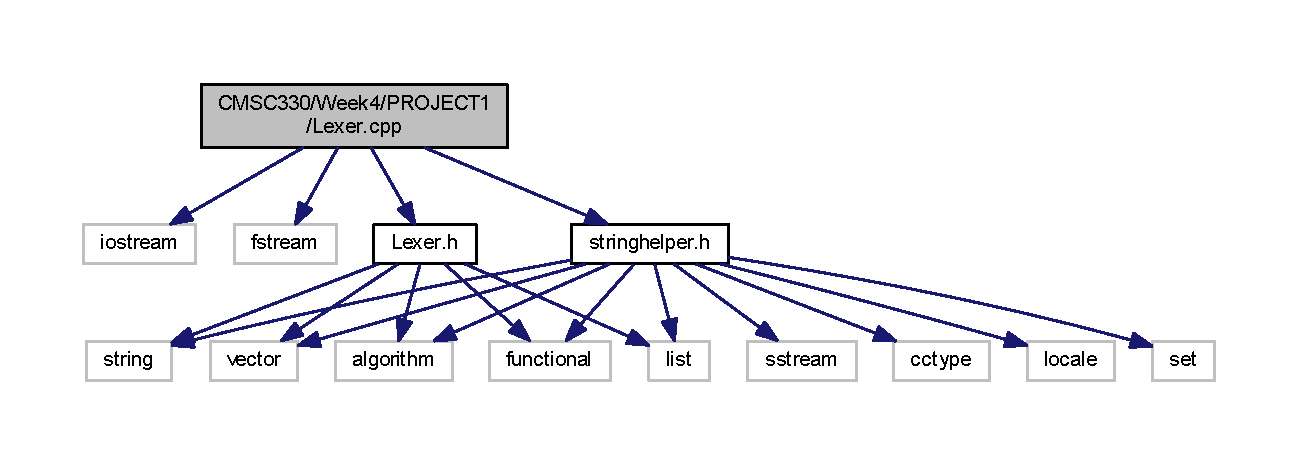
\includegraphics[width=350pt]{de/dd1/_lexer_8cpp__incl}
\end{center}
\end{figure}
\subsection*{Functions}
\begin{DoxyCompactItemize}
\item 
bool \hyperlink{_lexer_8cpp_a599876927aad28235b1608430dfd32ab}{check\+Number} (string number)
\end{DoxyCompactItemize}


\subsection{Detailed Description}
\begin{DoxyAuthor}{Author}
Kristopher Bickmore 
\end{DoxyAuthor}
\begin{DoxyDate}{Date}
November 21, 2016 
\end{DoxyDate}
\begin{DoxyRefDesc}{Bug}
\item[\hyperlink{bug__bug000001}{Bug}]No known bugs at this time \end{DoxyRefDesc}


\subsection{Function Documentation}
\hypertarget{_lexer_8cpp_a599876927aad28235b1608430dfd32ab}{}\label{_lexer_8cpp_a599876927aad28235b1608430dfd32ab} 
\index{Lexer.\+cpp@{Lexer.\+cpp}!check\+Number@{check\+Number}}
\index{check\+Number@{check\+Number}!Lexer.\+cpp@{Lexer.\+cpp}}
\subsubsection{\texorpdfstring{check\+Number()}{checkNumber()}}
{\footnotesize\ttfamily bool check\+Number (\begin{DoxyParamCaption}\item[{string}]{number }\end{DoxyParamCaption})}

Utility function used to check if a string is a valid number 
\begin{DoxyParams}{Parameters}
{\em number} & the string that may be a number \\
\hline
\end{DoxyParams}
\begin{DoxyReturn}{Returns}
true if a number, false otherwise 
\end{DoxyReturn}

\hypertarget{_lexer_8h}{}\section{C\+M\+S\+C330/\+Week4/\+P\+R\+O\+J\+E\+C\+T1/\+Lexer.h File Reference}
\label{_lexer_8h}\index{C\+M\+S\+C330/\+Week4/\+P\+R\+O\+J\+E\+C\+T1/\+Lexer.\+h@{C\+M\+S\+C330/\+Week4/\+P\+R\+O\+J\+E\+C\+T1/\+Lexer.\+h}}


Contains the \hyperlink{class_lexer}{Lexer} class definition.  


Include dependency graph for Lexer.\+h\+:
\nopagebreak
\begin{figure}[H]
\begin{center}
\leavevmode
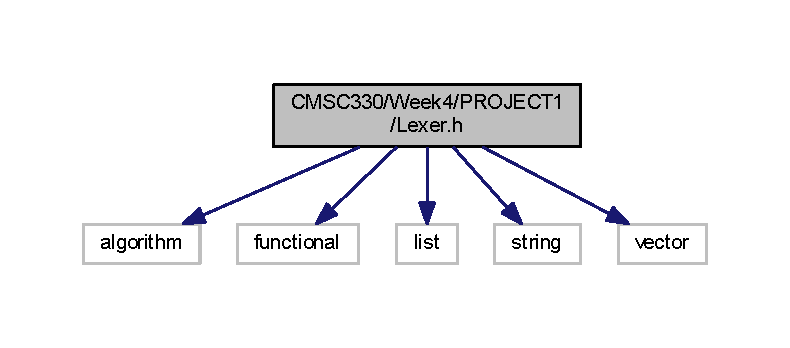
\includegraphics[width=350pt]{d8/de7/_lexer_8h__incl}
\end{center}
\end{figure}
This graph shows which files directly or indirectly include this file\+:
\nopagebreak
\begin{figure}[H]
\begin{center}
\leavevmode
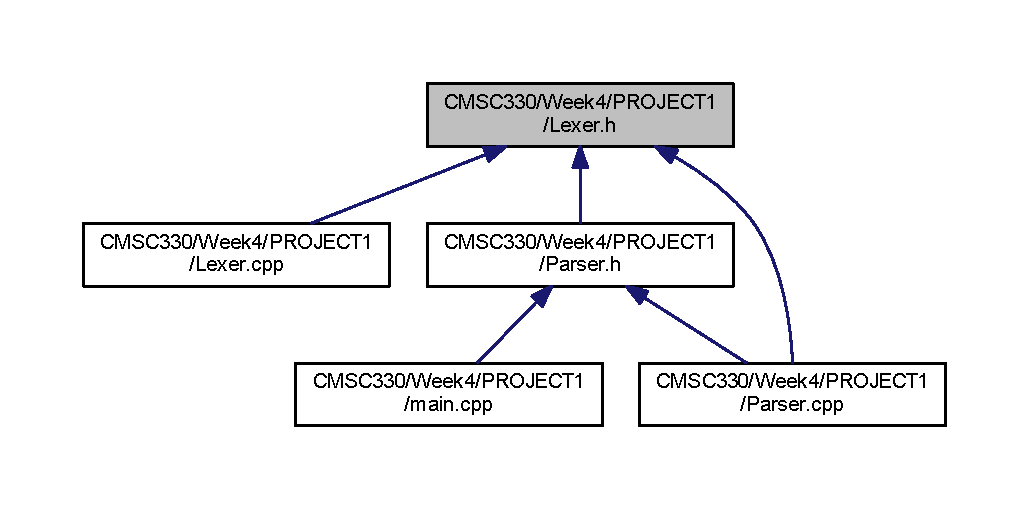
\includegraphics[width=350pt]{db/dbd/_lexer_8h__dep__incl}
\end{center}
\end{figure}
\subsection*{Classes}
\begin{DoxyCompactItemize}
\item 
class \hyperlink{class_lexer}{Lexer}
\begin{DoxyCompactList}\small\item\em This class is used to Lex a specific grammar\+: \end{DoxyCompactList}\end{DoxyCompactItemize}
\subsection*{Enumerations}
\begin{DoxyCompactItemize}
\item 
enum \hyperlink{_lexer_8h_a6a9e93b081bad7fc74c17306fb168c1f}{Token} \{ \newline
{\bfseries W\+I\+N\+D\+OW}, 
{\bfseries S\+T\+R\+I\+NG}, 
{\bfseries L\+A\+Y\+O\+UT}, 
{\bfseries O\+P\+E\+N\+P\+A\+R\+EN}, 
\newline
{\bfseries C\+L\+O\+S\+E\+P\+A\+R\+EN}, 
{\bfseries C\+O\+L\+ON}, 
{\bfseries S\+E\+M\+I\+C\+O\+L\+ON}, 
{\bfseries F\+L\+OW}, 
\newline
{\bfseries B\+O\+R\+D\+ER}, 
{\bfseries G\+R\+ID}, 
{\bfseries L\+E\+FT}, 
{\bfseries R\+I\+G\+HT}, 
\newline
{\bfseries C\+E\+N\+T\+ER}, 
{\bfseries B\+U\+T\+T\+ON}, 
{\bfseries G\+R\+O\+UP}, 
{\bfseries L\+A\+B\+EL}, 
\newline
{\bfseries P\+A\+N\+EL}, 
{\bfseries T\+E\+X\+T\+F\+I\+E\+LD}, 
{\bfseries R\+A\+D\+IO}, 
{\bfseries E\+ND}, 
\newline
{\bfseries P\+E\+R\+I\+OD}, 
{\bfseries N\+O\+NE}, 
{\bfseries E\+N\+D\+O\+F\+L\+I\+NE}, 
{\bfseries E\+N\+D\+O\+F\+F\+I\+LE}, 
\newline
{\bfseries N\+U\+M\+B\+ER}, 
{\bfseries C\+O\+M\+MA}
 \}
\end{DoxyCompactItemize}


\subsection{Detailed Description}
\begin{DoxyAuthor}{Author}
Kristopher Bickmore 
\end{DoxyAuthor}
\begin{DoxyDate}{Date}
November 11, 2016 
\end{DoxyDate}


\subsection{Enumeration Type Documentation}
\hypertarget{_lexer_8h_a6a9e93b081bad7fc74c17306fb168c1f}{}\label{_lexer_8h_a6a9e93b081bad7fc74c17306fb168c1f} 
\index{Lexer.\+h@{Lexer.\+h}!Token@{Token}}
\index{Token@{Token}!Lexer.\+h@{Lexer.\+h}}
\subsubsection{\texorpdfstring{Token}{Token}}
{\footnotesize\ttfamily enum \hyperlink{_lexer_8h_a6a9e93b081bad7fc74c17306fb168c1f}{Token}}

This enumeration contains all Tokens used in the associated grammar. 
\hypertarget{main_8cpp}{}\section{C\+M\+S\+C330/\+Week4/\+P\+R\+O\+J\+E\+C\+T1/main.cpp File Reference}
\label{main_8cpp}\index{C\+M\+S\+C330/\+Week4/\+P\+R\+O\+J\+E\+C\+T1/main.\+cpp@{C\+M\+S\+C330/\+Week4/\+P\+R\+O\+J\+E\+C\+T1/main.\+cpp}}


The driver for the parser application.  


Include dependency graph for main.\+cpp\+:
\nopagebreak
\begin{figure}[H]
\begin{center}
\leavevmode
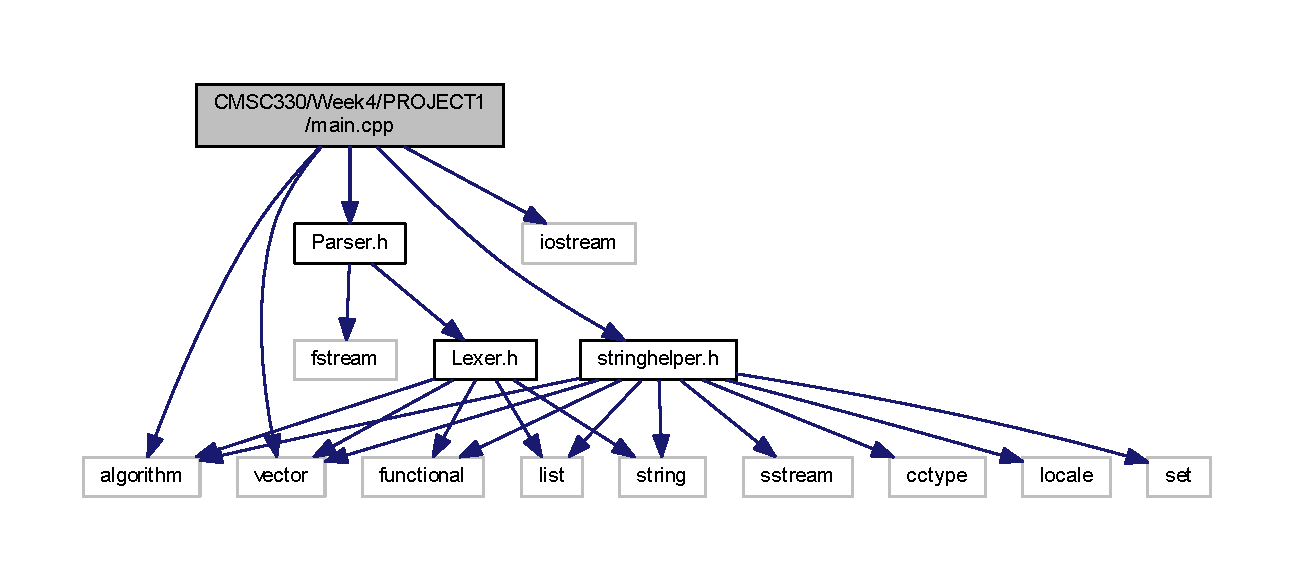
\includegraphics[width=350pt]{da/dce/main_8cpp__incl}
\end{center}
\end{figure}
\subsection*{Functions}
\begin{DoxyCompactItemize}
\item 
static void \hyperlink{main_8cpp_a64a8a9b12c7399fe0121c7c9397617b1}{show\+\_\+usage} (string name)
\item 
int \hyperlink{main_8cpp_a0ddf1224851353fc92bfbff6f499fa97}{main} (int argc, char $\ast$argv\mbox{[}$\,$\mbox{]})
\end{DoxyCompactItemize}


\subsection{Detailed Description}
\begin{DoxyAuthor}{Author}
Kristopher Bickmore 
\end{DoxyAuthor}
\begin{DoxyDate}{Date}
November 20, 2016 
\end{DoxyDate}


\subsection{Function Documentation}
\hypertarget{main_8cpp_a0ddf1224851353fc92bfbff6f499fa97}{}\label{main_8cpp_a0ddf1224851353fc92bfbff6f499fa97} 
\index{main.\+cpp@{main.\+cpp}!main@{main}}
\index{main@{main}!main.\+cpp@{main.\+cpp}}
\subsubsection{\texorpdfstring{main()}{main()}}
{\footnotesize\ttfamily int main (\begin{DoxyParamCaption}\item[{int}]{argc,  }\item[{char $\ast$}]{argv\mbox{[}$\,$\mbox{]} }\end{DoxyParamCaption})}

The main driver for the application 
\begin{DoxyParams}{Parameters}
{\em argc} & number of arguments \\
\hline
{\em argv} & the array of arguments \\
\hline
\end{DoxyParams}
\begin{DoxyReturn}{Returns}
an int 
\end{DoxyReturn}
\hypertarget{main_8cpp_a64a8a9b12c7399fe0121c7c9397617b1}{}\label{main_8cpp_a64a8a9b12c7399fe0121c7c9397617b1} 
\index{main.\+cpp@{main.\+cpp}!show\+\_\+usage@{show\+\_\+usage}}
\index{show\+\_\+usage@{show\+\_\+usage}!main.\+cpp@{main.\+cpp}}
\subsubsection{\texorpdfstring{show\+\_\+usage()}{show\_usage()}}
{\footnotesize\ttfamily static void show\+\_\+usage (\begin{DoxyParamCaption}\item[{string}]{name }\end{DoxyParamCaption})\hspace{0.3cm}{\ttfamily [static]}}

Prints a usage string to let the user know the available options. 
\begin{DoxyParams}{Parameters}
{\em name} & the name of the program. \\
\hline
\end{DoxyParams}

\hypertarget{_parser_8cpp}{}\section{C\+M\+S\+C330/\+Week4/\+P\+R\+O\+J\+E\+C\+T1/\+Parser.cpp File Reference}
\label{_parser_8cpp}\index{C\+M\+S\+C330/\+Week4/\+P\+R\+O\+J\+E\+C\+T1/\+Parser.\+cpp@{C\+M\+S\+C330/\+Week4/\+P\+R\+O\+J\+E\+C\+T1/\+Parser.\+cpp}}


Contains the source code for the \hyperlink{class_parser}{Parser} class.  


Include dependency graph for Parser.\+cpp\+:
\nopagebreak
\begin{figure}[H]
\begin{center}
\leavevmode
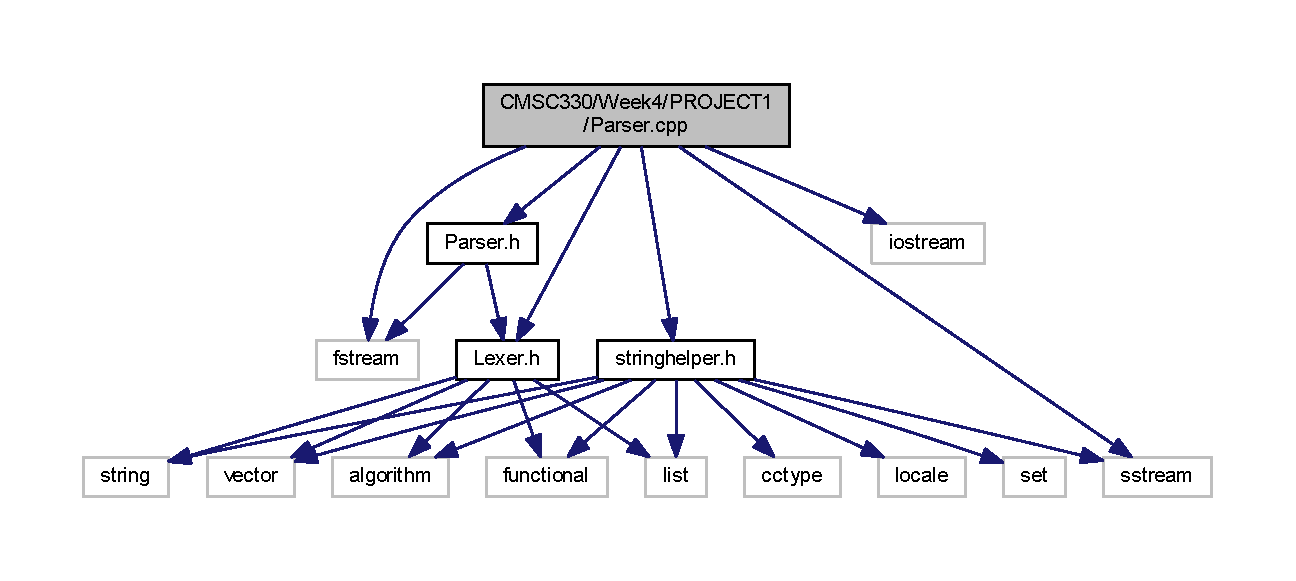
\includegraphics[width=350pt]{d6/d73/_parser_8cpp__incl}
\end{center}
\end{figure}
\subsection*{Macros}
\begin{DoxyCompactItemize}
\item 
\#define \hyperlink{_parser_8cpp_a2dc158afb0b9181c7ddc4e80b301c4de}{W\+R\+I\+T\+E\+\_\+\+L\+I\+NE}(writevalue)
\item 
\#define \hyperlink{_parser_8cpp_a32f584d1b4b908e205becafaaf5b35e2}{P\+A\+R\+S\+E\+R\+\_\+\+C\+H\+E\+CK}(C\+O\+ND)
\item 
\#define \hyperlink{_parser_8cpp_aa23b742766deca040a8e8b41bb6ad3f6}{P\+R\+O\+D\+U\+C\+T\+I\+O\+N\+\_\+\+C\+H\+E\+CK}(C\+O\+ND)
\end{DoxyCompactItemize}


\subsection{Detailed Description}
\begin{DoxyAuthor}{Author}
Kristopher Bickmore 
\end{DoxyAuthor}
\begin{DoxyDate}{Date}
November 20, 2016 
\end{DoxyDate}


\subsection{Macro Definition Documentation}
\hypertarget{_parser_8cpp_a32f584d1b4b908e205becafaaf5b35e2}{}\label{_parser_8cpp_a32f584d1b4b908e205becafaaf5b35e2} 
\index{Parser.\+cpp@{Parser.\+cpp}!P\+A\+R\+S\+E\+R\+\_\+\+C\+H\+E\+CK@{P\+A\+R\+S\+E\+R\+\_\+\+C\+H\+E\+CK}}
\index{P\+A\+R\+S\+E\+R\+\_\+\+C\+H\+E\+CK@{P\+A\+R\+S\+E\+R\+\_\+\+C\+H\+E\+CK}!Parser.\+cpp@{Parser.\+cpp}}
\subsubsection{\texorpdfstring{P\+A\+R\+S\+E\+R\+\_\+\+C\+H\+E\+CK}{PARSER\_CHECK}}
{\footnotesize\ttfamily \#define P\+A\+R\+S\+E\+R\+\_\+\+C\+H\+E\+CK(\begin{DoxyParamCaption}\item[{}]{C\+O\+ND }\end{DoxyParamCaption})}

{\bfseries Value\+:}
\begin{DoxyCode}
\textcolor{keywordflow}{if}(COND)\{ \(\backslash\)
        writeTokenLexeme(token, lexer.getCurrentLexeme());\(\backslash\)
        token = lexer.getNextToken(); \(\backslash\)
    \} \(\backslash\)
    else\{ \(\backslash\)
        ret = \textcolor{keyword}{false};\(\backslash\)
        goto cleanup;\(\backslash\)
    \}
\end{DoxyCode}
takes a conditional that compares the current token to the expected token value. If the token is valid syntactically then the process continues by writing the values and getting the next token. Otherwise the process fails. \hypertarget{_parser_8cpp_aa23b742766deca040a8e8b41bb6ad3f6}{}\label{_parser_8cpp_aa23b742766deca040a8e8b41bb6ad3f6} 
\index{Parser.\+cpp@{Parser.\+cpp}!P\+R\+O\+D\+U\+C\+T\+I\+O\+N\+\_\+\+C\+H\+E\+CK@{P\+R\+O\+D\+U\+C\+T\+I\+O\+N\+\_\+\+C\+H\+E\+CK}}
\index{P\+R\+O\+D\+U\+C\+T\+I\+O\+N\+\_\+\+C\+H\+E\+CK@{P\+R\+O\+D\+U\+C\+T\+I\+O\+N\+\_\+\+C\+H\+E\+CK}!Parser.\+cpp@{Parser.\+cpp}}
\subsubsection{\texorpdfstring{P\+R\+O\+D\+U\+C\+T\+I\+O\+N\+\_\+\+C\+H\+E\+CK}{PRODUCTION\_CHECK}}
{\footnotesize\ttfamily \#define P\+R\+O\+D\+U\+C\+T\+I\+O\+N\+\_\+\+C\+H\+E\+CK(\begin{DoxyParamCaption}\item[{}]{C\+O\+ND }\end{DoxyParamCaption})}

{\bfseries Value\+:}
\begin{DoxyCode}
\textcolor{keywordflow}{if}(!COND)\{\(\backslash\)
        ret = \textcolor{keyword}{false};\(\backslash\)
        goto cleanup;\(\backslash\)
    \}
\end{DoxyCode}
takes a conditional that compares whether a production function succeeded or not. \hypertarget{_parser_8cpp_a2dc158afb0b9181c7ddc4e80b301c4de}{}\label{_parser_8cpp_a2dc158afb0b9181c7ddc4e80b301c4de} 
\index{Parser.\+cpp@{Parser.\+cpp}!W\+R\+I\+T\+E\+\_\+\+L\+I\+NE@{W\+R\+I\+T\+E\+\_\+\+L\+I\+NE}}
\index{W\+R\+I\+T\+E\+\_\+\+L\+I\+NE@{W\+R\+I\+T\+E\+\_\+\+L\+I\+NE}!Parser.\+cpp@{Parser.\+cpp}}
\subsubsection{\texorpdfstring{W\+R\+I\+T\+E\+\_\+\+L\+I\+NE}{WRITE\_LINE}}
{\footnotesize\ttfamily \#define W\+R\+I\+T\+E\+\_\+\+L\+I\+NE(\begin{DoxyParamCaption}\item[{}]{writevalue }\end{DoxyParamCaption})}

{\bfseries Value\+:}
\begin{DoxyCode}
\textcolor{keywordflow}{if}(print)\{\(\backslash\)
        cout << writevalue << endl;\(\backslash\)
    \}\(\backslash\)
    outfile << writevalue << endl;
\end{DoxyCode}
Writes a string to to the parser\textquotesingle{}s ofstream, also prints to stdout if print is true. 
\begin{DoxyParams}{Parameters}
{\em writevalue} & \\
\hline
\end{DoxyParams}

\hypertarget{_parser_8h}{}\section{C\+M\+S\+C330/\+Week4/\+P\+R\+O\+J\+E\+C\+T1/\+Parser.h File Reference}
\label{_parser_8h}\index{C\+M\+S\+C330/\+Week4/\+P\+R\+O\+J\+E\+C\+T1/\+Parser.\+h@{C\+M\+S\+C330/\+Week4/\+P\+R\+O\+J\+E\+C\+T1/\+Parser.\+h}}


Contains the \hyperlink{class_parser}{Parser} Class definition.  


Include dependency graph for Parser.\+h\+:
\nopagebreak
\begin{figure}[H]
\begin{center}
\leavevmode
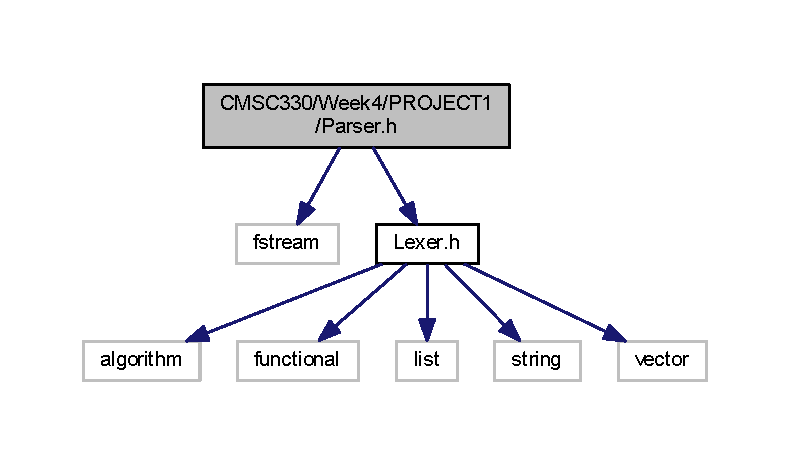
\includegraphics[width=350pt]{d6/d7e/_parser_8h__incl}
\end{center}
\end{figure}
This graph shows which files directly or indirectly include this file\+:
\nopagebreak
\begin{figure}[H]
\begin{center}
\leavevmode
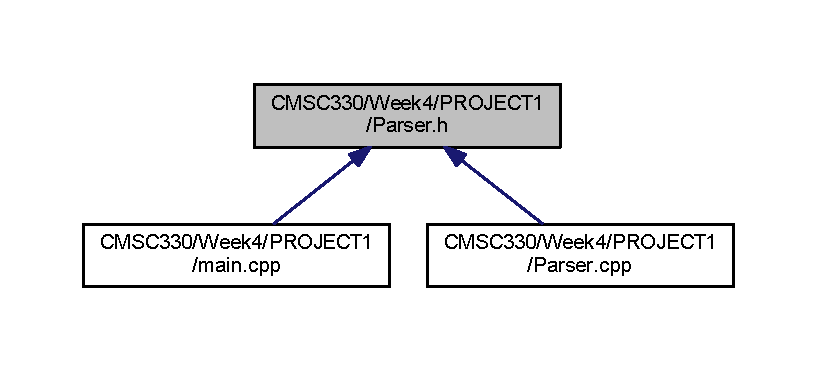
\includegraphics[width=350pt]{d1/d33/_parser_8h__dep__incl}
\end{center}
\end{figure}
\subsection*{Classes}
\begin{DoxyCompactItemize}
\item 
class \hyperlink{class_parser}{Parser}
\begin{DoxyCompactList}\small\item\em The parser class parses a specific grammar. \end{DoxyCompactList}\end{DoxyCompactItemize}


\subsection{Detailed Description}
\begin{DoxyAuthor}{Author}
Kristopher Bickmore 
\end{DoxyAuthor}
\begin{DoxyDate}{Date}
November 20, 2016 
\end{DoxyDate}

\hypertarget{stringhelper_8h}{}\section{C\+M\+S\+C330/\+Week4/\+P\+R\+O\+J\+E\+C\+T1/stringhelper.h File Reference}
\label{stringhelper_8h}\index{C\+M\+S\+C330/\+Week4/\+P\+R\+O\+J\+E\+C\+T1/stringhelper.\+h@{C\+M\+S\+C330/\+Week4/\+P\+R\+O\+J\+E\+C\+T1/stringhelper.\+h}}


Contains the definition and source code for the \hyperlink{class_string_helper}{String\+Helper} class which provides extra string functionality.  


Include dependency graph for stringhelper.\+h\+:
\nopagebreak
\begin{figure}[H]
\begin{center}
\leavevmode
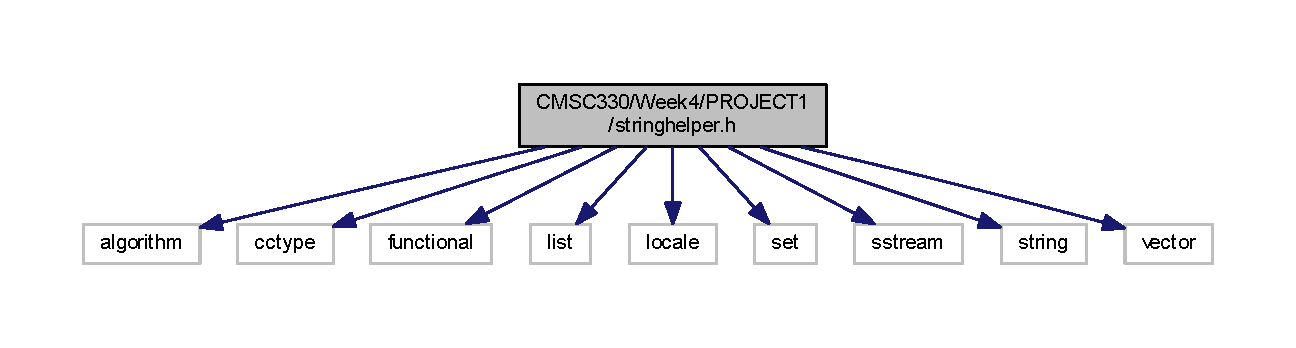
\includegraphics[width=350pt]{d1/d5b/stringhelper_8h__incl}
\end{center}
\end{figure}
This graph shows which files directly or indirectly include this file\+:
\nopagebreak
\begin{figure}[H]
\begin{center}
\leavevmode
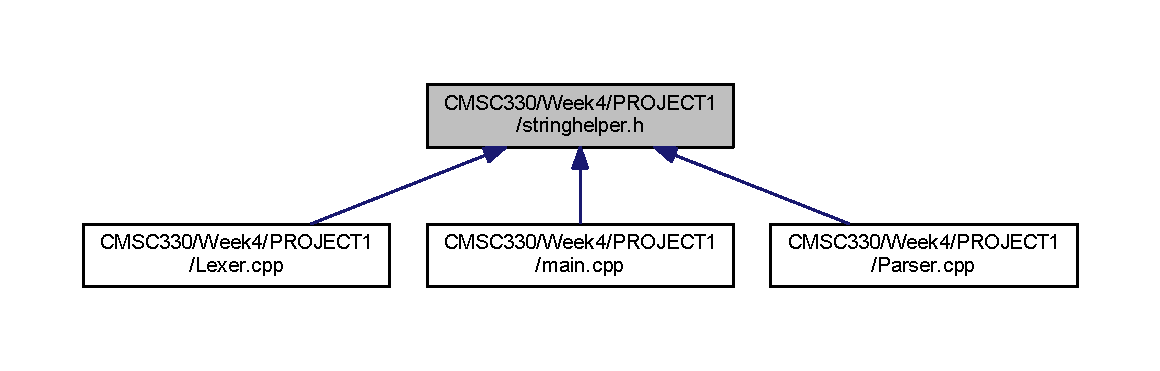
\includegraphics[width=350pt]{dc/d04/stringhelper_8h__dep__incl}
\end{center}
\end{figure}
\subsection*{Classes}
\begin{DoxyCompactItemize}
\item 
class \hyperlink{class_string_helper}{String\+Helper}
\begin{DoxyCompactList}\small\item\em This class assists in handling std\+::string variables. \end{DoxyCompactList}\end{DoxyCompactItemize}


\subsection{Detailed Description}
\begin{DoxyAuthor}{Author}
Kristopher Bickmore 
\end{DoxyAuthor}
\begin{DoxyDate}{Date}
November 20, 2016 
\end{DoxyDate}

%--- End generated contents ---

% Index
\backmatter
\newpage
\phantomsection
\clearemptydoublepage
\addcontentsline{toc}{chapter}{Index}
\printindex

\end{document}
